\documentclass{beamer}
\usepackage{graphicx}
\usepackage{xcolor}
\usepackage{tikz}
\usepackage{amsmath}
\usepackage{pgfplots}
\pgfplotsset{compat=1.18}

\definecolor{purpleblue}{RGB}{80, 80, 180}
\definecolor{novelPurple}{RGB}{98, 54, 255}
\definecolor{softPurple}{RGB}{180, 170, 255}
\definecolor{softGray}{RGB}{235, 235, 245}
\definecolor{lightText}{RGB}{90, 90, 110}

\usetheme{Madrid}
\usecolortheme{dolphin}
\graphicspath{{static/course_materials/}{static/hard/}{./}}

\setbeamerfont{title}{size=\Large,series=\bfseries}
\setbeamerfont{frametitle}{size=\LARGE,series=\bfseries}
\setbeamercolor{frametitle}{fg=white, bg=novelPurple}
\setbeamercolor{title}{fg=white, bg=purpleblue}

\title[Final Review]{\textbf{Final Review}}
\author{\textbf{Jack Zeng}}
\institute{\textcolor{white}{\textbf{Novel Prep}}}
\date{\today}

\begin{document}

\begin{frame}
    \titlepage
    \vfill
    \begin{flushright}
        \textcolor{purpleblue}{\Huge \textbf{Novel Prep}}
    \end{flushright}
\end{frame}

\begin{frame}
    \begin{tikzpicture}[remember picture, overlay]
        \shade[top color=softPurple, bottom color=softGray]
            (current page.north west) rectangle (current page.south east);
        \node[align=center] at (current page.center) {
            {\Huge\bfseries\textcolor{purpleblue}{Novel Prep}} \\[0.5cm]
            {\Large\itshape\textcolor{lightText}{Phase 3 · Final Review}}
        };
    \end{tikzpicture}
\end{frame}

\begin{frame}{Overview}
    \tableofcontents
\end{frame}

\begin{frame}
\section{Final Review}
    \begin{tikzpicture}[remember picture, overlay]
        \shade[top color=softPurple, bottom color=softGray]
            (current page.north west) rectangle (current page.south east);
        \node[align=center] at (current page.center) {
            {\LARGE\bfseries\textcolor{purpleblue}{Final Review}} \\[0.5cm]
            {\Large\itshape\textcolor{lightText}{11 Phase 3 final review questions}}
        };
    \end{tikzpicture}
\end{frame}

% --- Question 1 ---
\begin{frame}{Question 1}
\small
In the given equation, \(k\) is a constant. The equation has exactly one real solution. What is the value of \(k\)?
\[
x^{2} + \bigl(\sqrt{k - 3}\bigr)x + 42 = 0
\]
\vspace{0.35cm}
\begin{enumerate}
    \item[A.] \(171\)
    \item[B.] \(168\)
    \item[C.] \(165\)
    \item[D.] \(45\)
\end{enumerate}
\end{frame}
\begin{frame}{Answer 1}
\small
\textbf{Correct Answer:} A
\end{frame}

% --- Question 2 ---
\begin{frame}{Question 2}
\small
In the given system of equations, \(m\) and \(b\) are negative constants. In the \(xy\)-plane, the graphs of the equations in the given system intersect at the point \((-5, y)\), where \(y < 0\). Which expression represents the value of \(b\)?
\[
\begin{aligned}
x^{2} + y^{2} &= 36 \\
y &= mx + \dfrac{b}{4}
\end{aligned}
\]
\vspace{0.35cm}
\begin{enumerate}
    \item[A.] \(-\dfrac{5m}{4} + \dfrac{\sqrt{11}}{4}\)
    \item[B.] \(\dfrac{5m}{4} - \dfrac{\sqrt{11}}{4}\)
    \item[C.] \(-20m + 4\sqrt{11}\)
    \item[D.] \(20m - 4\sqrt{11}\)
\end{enumerate}
\end{frame}
\begin{frame}{Answer 2}
\small
\textbf{Correct Answer:} D
\end{frame}

% --- Question 3 ---
\begin{frame}{Question 3}
\small
A biologist mixed a solution that is \(0.3\%\) sodium chloride by mass with a solution that is \(0.15\%\) sodium chloride by mass to obtain a new solution, which has a mass of \(80\) grams and contains \(0.21\) grams of sodium chloride. How many grams of \(0.3\%\) sodium chloride solution did the biologist use?
\vspace{0.35cm}
\begin{enumerate}
    \item[A.] \(0.14\)
    \item[B.] \(20\)
    \item[C.] \(60\)
    \item[D.] \(79.86\)
\end{enumerate}
\end{frame}
\begin{frame}{Answer 3}
\small
\textbf{Correct Answer:} C
\end{frame}

% --- Question 4 ---
\begin{frame}{Question 4}
\small
The function \(v\) is defined by the equation
\[
v(x) = \dfrac{x^{2} + bx + c}{(x + 5)(x - 19)},
\]
where \(b\) and \(c\) are constants. In the \(xy\)-plane, the graph of \(y = v(x)\) passes through the points \(\bigl(0, \dfrac{66}{95}\bigr)\) and \((11, 0)\). If \(v(q) = 0\), which of the following could be the value of \(q\)?
\vspace{0.35cm}
\begin{enumerate}
    \item[A.] \(-6\)
    \item[B.] \(-5\)
    \item[C.] \(5\)
    \item[D.] \(6\)
\end{enumerate}
\end{frame}
\begin{frame}{Answer 4}
\small
\textbf{Correct Answer:} A
\end{frame}

% --- Question 5 ---
\begin{frame}{Question 5}
\small
\[
\dfrac{x}{5} + \dfrac{y}{9} = \dfrac{47}{45}
\]
An engineer connects resistors in series, where the resistors in the series have a total resistance of \(\dfrac{47}{45}\) ohms. In this series, there are \(x\) resistors of type A, which each have a resistance of \(a\) ohms, and \(y\) resistors of type B, which each have a resistance of \(b\) ohms. The given equation represents this situation. According to this equation, what is the positive difference between the value of \(a\) and the value of \(b\)?
\vspace{0.35cm}
\begin{enumerate}
    \item[A.] \(47\)
    \item[B.] \(4\)
    \item[C.] \(\dfrac{47}{45}\)
    \item[D.] \(\dfrac{4}{45}\)
\end{enumerate}
\end{frame}
\begin{frame}{Answer 5}
\small
\textbf{Correct Answer:} D
\end{frame}

% --- Question 6 ---
\begin{frame}{Question 6}
\small
\begin{center}
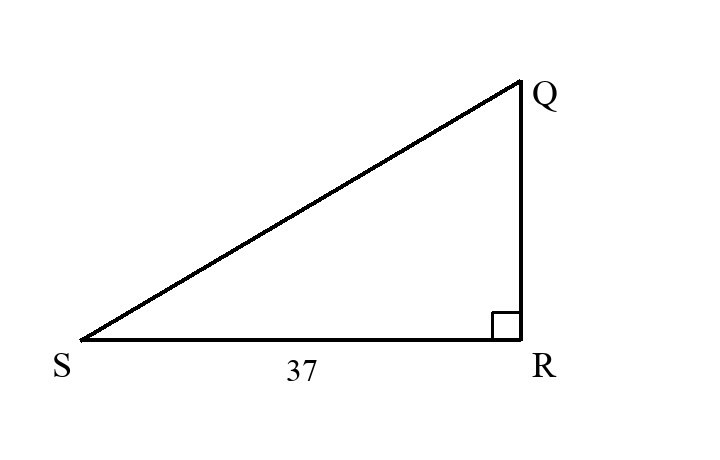
\includegraphics[width=0.62\linewidth]{hard_30_f06_triangle.png}
\end{center}
{\footnotesize Note: Figure not drawn to scale.}

In triangle \(QRS\) shown, \(QR < RS\). Which expression represents the length of \(\overline{QS}\)?
\vspace{0.35cm}
\begin{enumerate}
    \item[A.] \(37\cos Q\)
    \item[B.] \(37\sin Q\)
    \item[C.] \(\dfrac{37}{\cos Q}\)
    \item[D.] \(\dfrac{37}{\sin Q}\)
\end{enumerate}
\end{frame}
\begin{frame}{Answer 6}
\small
\textbf{Correct Answer:} D
\end{frame}

% --- Question 7 ---
\begin{frame}{Question 7}
\small
A group of \(10\) gardeners recorded data on the germination rates of their tomato crop for one growing season. The scatterplot shows the relationship between the number of tomato seeds planted, \(x\), and the number of tomato seeds that germinated, \(y\), for each of the gardeners. A line of best fit is also shown.

\begin{center}
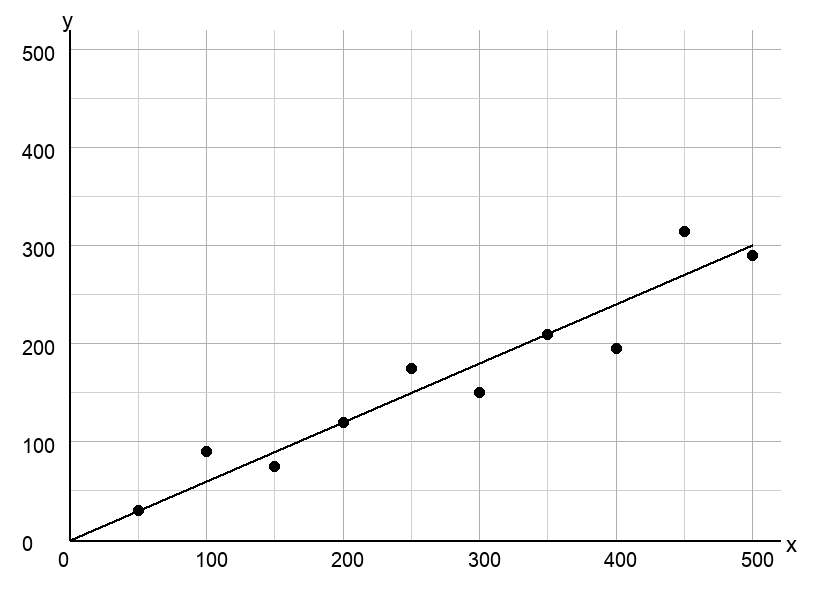
\includegraphics[width=0.78\linewidth]{hard_30_f07_scatter.png}
\end{center}

Which of the following is the best interpretation of the slope of the line of best fit in this context?
\vspace{0.35cm}
\begin{enumerate}
    \item[A.] The number of tomato seeds planted is predicted to increase by \(60\) seeds every \(100\) days.
    \item[B.] The number of tomato seeds planted is predicted to increase by \(300\) seeds every \(100\) days.
    \item[C.] The number of tomato seeds that germinate is predicted to increase by \(60\) seeds for every additional \(100\) tomato seeds that are planted.
    \item[D.] The number of tomato seeds that germinate is predicted to increase by \(300\) seeds for every additional \(100\) tomato seeds that are planted.
\end{enumerate}
\end{frame}
\begin{frame}{Answer 7}
\small
\textbf{Correct Answer:} C
\end{frame}

% --- Question 8 ---
\begin{frame}{Question 8}
\small
A rectangular banner has an area of \(3{,}200\) square inches. A copy of the banner is made in which the length and width of the original banner are each increased by \(20\%\). What is the area of the copy, in square inches?
\vspace{0.35cm}
\begin{enumerate}
    \item[A.] \(3{,}220\)
    \item[B.] \(3{,}240\)
    \item[C.] \(3{,}840\)
    \item[D.] \(4{,}608\)
\end{enumerate}
\end{frame}
\begin{frame}{Answer 8}
\small
\textbf{Correct Answer:} D
\end{frame}

% --- Question 9 ---
\begin{frame}{Question 9}
\small
The mass of object A is \(444\%\) of the mass of object B, and the mass of object A is \(0.740\%\) of the mass of object C. If the mass of object C is \(p\%\) of the mass of object B, what is the value of \(p\)?
\end{frame}
\begin{frame}{Answer 9}
\small
\textbf{Final Answer:} $\boxed{60000}$
\end{frame}

% --- Question 10 ---
\begin{frame}{Question 10}
\small
In \(2013\), Chloe earned \(11\%\) more than in \(2012\), and in \(2014\) Chloe earned \(6\%\) more than in \(2013\). If Chloe earned \(y\) times as much in \(2012\) as in \(2014\), which of the following is closest to the value of \(y\)?
\vspace{0.35cm}
\begin{enumerate}
    \item[A.] \(0.5455\)
    \item[B.] \(0.6600\)
    \item[C.] \(0.8499\)
    \item[D.] \(1.1766\)
\end{enumerate}
\end{frame}
\begin{frame}{Answer 10}
\small
\textbf{Correct Answer:} C
\end{frame}

% --- Question 11 ---
\begin{frame}{Question 11}
\small
Point \(F\) lies on a unit circle in the \(xy\)-plane and has coordinates \((1, 0)\). Point \(G\) is the center of the circle and has coordinates \((0, 0)\). Point \(H\) also lies on the circle and has coordinates \((-1, y)\), where \(y\) is a constant. Which of the following could be the positive measure of angle \(FGH\), in radians?
\vspace{0.35cm}
\begin{enumerate}
    \item[A.] \(\dfrac{37\pi}{2}\)
    \item[B.] \(\dfrac{39\pi}{2}\)
    \item[C.] \(34\pi\)
    \item[D.] \(35\pi\)
\end{enumerate}
\end{frame}
\begin{frame}{Answer 11}
\small
\textbf{Correct Answer:} D
\end{frame}

% --- Phase 3 final student advice ---
\newcommand{\AdviceTip}[3]{%
\noindent\begin{minipage}{\linewidth}
\begin{tikzpicture}
\node[
  rounded corners=8pt,
  fill=white,
  draw=novelPurple!22,
  line width=0.6pt,
  inner xsep=10pt,
  inner ysep=7pt,
  text width=\dimexpr\linewidth-22pt\relax,
  align=flush left
] (card) {%
  {\color{novelPurple}\bfseries\small #1~~#2}\\[0.15em]
  {\scriptsize\textcolor{lightText}{#3}}%
};
\fill[novelPurple] (card.south west) rectangle ([xshift=3pt]card.north west);
\end{tikzpicture}%
\end{minipage}\vspace{0.22em}%
}

\begin{frame}[plain]{Final Advice · Phase 3}
\begin{tikzpicture}[remember picture, overlay]
  \shade[top color=softPurple!85, bottom color=white]
    (current page.north west) rectangle (current page.south east);
  \fill[novelPurple, opacity=0.08] ([yshift=-0.6cm]current page.north west)
    rectangle ([yshift=-2.35cm]current page.north east);
\end{tikzpicture}
\vspace{0.15em}
{\scriptsize\bfseries\textcolor{novelPurple}{PHASE 3 · LAST CLASS}}\\[0.2em]
{\LARGE\bfseries\textcolor{purpleblue}{Final Advice}}\\[0.12em]
{\footnotesize\textcolor{lightText}{Keep these habits with you after today.}}
\vspace{0.55em}

\AdviceTip{01}{Desmos is a tool, not a crutch}{%
Use Desmos for graphs, points, or quick arithmetic --- not for every question.
Many items are faster and safer with algebra or a short written setup.
Solve by hand when you can; use Desmos to verify when unsure.}

\AdviceTip{02}{Read the ask first, then harvest the stem}{%
Start with the last line: what is the question asking?
Then go line by line and ask, ``What math idea is this pointing to?''
Each line often hints at a formula, ratio, or constraint.
Capture the hints, choose a method, then compute.}

\AdviceTip{03}{Build speed without giving up accuracy}{%
Spend less time stuck on one item. Recognize the type and skill quickly.
If you are spinning, mark it, move on, and return later.
Accuracy first --- then faster recognition.}
\end{frame}

\begin{frame}[plain]{How to Prep From Here}
\begin{tikzpicture}[remember picture, overlay]
  \shade[top color=softPurple!85, bottom color=white]
    (current page.north west) rectangle (current page.south east);
  \fill[novelPurple, opacity=0.08] ([yshift=-0.6cm]current page.north west)
    rectangle ([yshift=-2.35cm]current page.north east);
\end{tikzpicture}
\vspace{0.15em}
{\scriptsize\bfseries\textcolor{novelPurple}{FROM HERE}}\\[0.2em]
{\LARGE\bfseries\textcolor{purpleblue}{How to Prep}}\\[0.12em]
{\footnotesize\textcolor{lightText}{Short, focused practice beats a long vague season.}}
\vspace{0.45em}

\begin{columns}[T]
\begin{column}{0.48\textwidth}
\AdviceTip{04}{Keep prep focused}{%
Use a short, concentrated block: drills, mocks, and review of misses.
You already have enough Novel Prep questions for SAT Math --- find gaps and fix them.}
\vspace{0.15em}
\AdviceTip{05}{Close the loop}{%
After each set, write 2--3 skills you missed.
Drill those next --- not the whole book again.}
\end{column}
\begin{column}{0.48\textwidth}
\AdviceTip{06}{Manage the clock}{%
Skip and return. Do not burn four minutes early on one hard problem.
Easy and medium points first.}
\vspace{0.15em}
\AdviceTip{07}{Trust your method}{%
Restate the ask, underline givens, eliminate choices, or plug in a number.
The habits from class are enough --- use them calmly.}
\end{column}
\end{columns}

\vspace{0.35em}
\centering

\begin{tikzpicture}
\node[
  rounded corners=10pt,
  fill=novelPurple!12,
  draw=novelPurple!28,
  inner xsep=14pt,
  inner ysep=7pt,
  font=\small\itshape
] {\textcolor{purpleblue}{Short prep. Clear method. Smart use of tools. You've got this.}};
\end{tikzpicture}
\end{frame}
\begin{frame}{}
    \begin{tikzpicture}[remember picture, overlay]
        \shade[top color=novelPurple!40, bottom color=white]
            (current page.north west) rectangle (current page.south east);
        \fill[white, opacity=0.15] (current page.center) circle (5cm);
        \foreach \x in {1,2,3,4,5} {
            \fill[novelPurple, opacity=0.12] (rand*10-5, rand*7-3.5) circle (0.1+\x*0.05);
        }
    \end{tikzpicture}
    \centering
    \vspace{5em}
    {\Huge \textbf{\textcolor{novelPurple}{Thank You!}}} \\[1em]
    {\large \textcolor{gray}{We appreciate your time and focus.}} \\[3em]
    {\LARGE \textbf{\textcolor{novelPurple}{\textsf{Novel Prep}}}}
    \vfill
\end{frame}

\end{document}
